% !TEX TS-program = pdflatex
% !TEX encoding = UTF-8 Unicode

% This is a simple template for a LaTeX document using the "article" class.
% See "book", "report", "letter" for other types of document.

\documentclass[11pt,twocolumn]{article} % use larger type; default would be 10pt

\usepackage[utf8]{inputenc} % set input encoding (not needed with XeLaTeX)

%%% Examples of Article customizations
% These packages are optional, depending whether you want the features they provide.
% See the LaTeX Companion or other references for full information.

%%% PAGE DIMENSIONS
\usepackage{geometry} % to change the page dimensions
\geometry{a4paper} % or letterpaper (US) or a5paper or....
% \geometry{margin=2in} % for example, change the margins to 2 inches all round
% \geometry{landscape} % set up the page for landscape
%   read geometry.pdf for detailed page layout information

\usepackage{graphicx} % support the \includegraphics command and options
\usepackage{mathtools}
\usepackage{amsmath} % need this stuff for curly brackets
% \usepackage[parfill]{parskip} % Activate to begin paragraphs with an empty line rather than an indent

%%% PACKAGES
\usepackage{booktabs} % for much better looking tables
\usepackage{array} % for better arrays (eg matrices) in maths
\usepackage{paralist} % very flexible & customisable lists (eg. enumerate/itemize, etc.)
\usepackage{verbatim} % adds environment for commenting out blocks of text & for better verbatim
\usepackage{subfig} % make it possible to include more than one captioned figure/table in a single float
\usepackage{authblk}
\usepackage{pdfpages}
\usepackage{wrapfig}
\usepackage{hyperref}
\usepackage{listings}
\lstset{frame=tb,
  language=BASH,
  aboveskip=3mm,
  belowskip=3mm,
  showstringspaces=false,
  columns=flexible,
  basicstyle={\small\ttfamily},
  numbers=none,
  numberstyle=\tiny\color{gray},
  keywordstyle=\color{blue},
  commentstyle=\color{dkgreen},
  stringstyle=\color{mauve},
  breaklines=true,
  breakatwhitespace=true
  tabsize=1
}
% These packages are all incorporated in the memoir class to one degree or another...

%%% HEADERS & FOOTERS
\usepackage{fancyhdr} % This should be set AFTER setting up the page geometry
\pagestyle{fancy} % options: empty , plain , fancy
\renewcommand{\headrulewidth}{0pt} % customise the layout...
\lhead{}\chead{}\rhead{}
\lfoot{}\cfoot{\thepage}\rfoot{}

%%% SECTION TITLE APPEARANCE
\usepackage{sectsty}
\allsectionsfont{\sffamily\mdseries\upshape} % (See the fntguide.pdf for font help)
% (This matches ConTeXt defaults)

%%% ToC (table of contents) APPEARANCE
\usepackage[nottoc,notlof,notlot]{tocbibind} % Put the bibliography in the ToC
\usepackage[titles,subfigure]{tocloft} % Alter the style of the Table of Contents
\renewcommand{\cftsecfont}{\rmfamily\mdseries\upshape}
\renewcommand{\cftsecpagefont}{\rmfamily\mdseries\upshape} % No bold!

%%% END Article customizations

\title{Software Engineering For Industry \\ AcmeTelecom - Report}
\author[1]{Dan Demeter\thanks{dan.demeter10@imperial.ac.uk}}
\author[1]{Dan Octavian\thanks{dan.octavian10@imperial.ac.uk}}
\author[1]{Razvan Rosie\thanks{razvan.rosie10@imperial.ac.uk}}
\author[1]{Marius Telespan\thanks{marius.telespan10@imperial.ac.uk}}
\affil[1]{Department of Computing, Imperial College London}

\begin{document}
\maketitle

\begin{abstract}
In our report we describe the newly designed software for the telecommunication company ACME Telecom. The main task was to improve the way 
user bills are calculated. Furthermore, we present a new way of organising the source code in a modular design fashion. 
Our solution makes use of the best software engineering practices, includes unit and acceptance tests.

Additionally, we have extended the initial solution by providing source code runnable on $Amazon'$ $Web$ $Services$ $Elastic$ $Map$ $Reduce$. As such, 
ACME Telecom will be prepared for a future scalability issue when dealing with large sets of customers .
\newline

{\bf Keywords}: acceptance testing, unit testing, design patterns, code refactoring, scalability.
\end{abstract}


\section{Introduction}
AcmeTelecom is a telecommunication company which is currently running calculating the pricing and billing calculations
for all of Acme's mobile phone customers in the following way: if a customer begins a call during the peak time, and the call 
continues in off-peak period, then the whole call is billed at the the peak rate. Similarly, if a customer the call starts in 
the off-peak period and finish in the peak time, the whole call is billed as being a peak time call. Any call that overlaps the 
peak time period is charged as a peak call.

Our main task was to rewrite the code making sure that the billing system is fair for every customer. In order to make sure that our changes work,
we added acceptance and unit tests covering the existing code.

This report is organized in the following way: {\bf Section 2} presents our implementation of the main feature of the program, which
allows to fairly compute the billings. {\bf Section 3} presents the way that the code was refactoring. 
{\bf Section 4} includes the addition features that were added. 
The fifth section gives an overview of the testing methodologies that were used during the project, together with the testing tools.
{\bf Section 6} discusses some design decisions that we have taken.
The last part of the report offers our concluding remarks and potential improvements for the code.

\section{ACME Telecom v2}

\subsection{Improved Cost Calculator}

The initial implementation for calculating the call costs was not taking correctly into consideration 
the $starting$ and $end$ times for a call. As a results, calls which were taking place during both $off$-$peak$ and 
$on$-$peak$ times were being charged for the entire duration with the $on$-$peak$ tariff. For example, for an $on$-$peak$
period of 7:00 $-$ 18:59, a call from 20:30 until 21:30 would be correctly charged for 60 minutes $\ast$
$off$-$peak$ tariff, but a call from  18:30 until 19:30 would be charged incorrectly 60 minutes $\ast$ \textbf{on-peak},
instead of 30 minutes $\ast$ \textbf{on-peak} $+$ 30 minutes $\ast$ \textbf{off-peak}.

Our code implementation solves this problem, and the algorithm can be described as follows. All $notations$ represented by capital letters 
are $DateTime$ (Joda library) instances:
\begin{enumerate}
\item{For the start call ($START$), find the next (\textit{higher}) \textit{peak/off-peak} time delimiter 
( 7:00 or 19:00 ) and save it as $T_1$.}

\item{For the end call ($END$), find the previous (\textit{lower}) \textit{peak/off-peak} time delimiter 
( 7:00 or 19:00 ) and save it as $T_2$.}

\item{Compute the seconds between $START$ and $T1$ (referred as $C_1$) and between $END$ and $T_2$ (referred as $C_2$).}


\end{enumerate}

$\bullet$ The case when $T_1 > T_2$ means that $START$ and $END$ times are in the same \textit{peak or off-peak} period. 
Trivially, we can then compute the cost for the call as ($END$ - $START$) $\ast$ (\textit{on-peak OR off-peak}) tariff. 
The tariff type can be easily found. 

$\bullet$ In all other cases, when $T_1 \leq T_2$, $START$ and $END$ may be in different zones. Therefore, we 
calculate how many 12 hours intervals are between $T_1$ and $T_2$. If that number is even,  we know that $\frac{1}{2}$ of that 
time the call should be charged with the \textit{off-peak} tariff, and the other $\frac{1}{2}$ time should be charged with the 
\textit{on-peak} time. In case that number is odd, then we identify the one extra period (depending if the call started in 
\textit{on-peak OR off-peak}) and which tariff should be applied to it.

$\bullet$ The final cost for a customer is: [the total cost for the set of 12 hours periods] $+$ [the cost between $START$ 
and $T_1$ ($C_1$)] $+$ [the cost between $T_2$ and $END$ ($C_2$)]. 
Again, for $C_1$ and $C_2$ we can easily identify what tariff we need to use: the \textit{peak or off-peak} one.

\subsection{Calls Longer than 24 Hours}

Due to our improved formula for computing the correct and fair cost (presented above), we have removed the initial issue 
of any call lasting longer than 24 hours. Our formula takes into consideration any length of time between the calls and 
with the help of our algorithm we can compute the exact cost in a linear time.

\subsection{Joda}
JodaTime helped us a lot in order to manage all the complexity for handling periods of time,
translating the a date into milliseconds and subtracting 2 different Dates. It was also extremely useful for manipulating 
different types of DateTime instances and operations.

\subsection{Printer}
In terms of generating the status of the bills for the customers, the system was directing its results to the Standard Output pipe. 
Unfortunately, the only present output interface (HtmlPrinter) was generating HTML tables which were not following the W3C standards. 
Because we have decided to make our system as reliable as possible, we had to take into consideration different environments where 
our system would be running: it could run on a server without any output attached (headless server), or for debugging purposes, 
the billing output should be easily read and parsed from the terminal. 
By using the \textit{abstract factory design pattern}, we have restructured our Output Interface as an abstract Class, 
having different classes extend it. These classes will be actual printing and formatting the results in a way suitable for the environment.
The current classes we have implemented or changed in the system are: HTMLPrinter and ConsolePrinter. HTMLPrinter is the initial 
implementation printing the results in an HTML format. We have decided \textbf{not} to change it, because some other legacy software 
might be parsing the HTML file generated by our system. This is a major risk, because we can't control how other software interacts 
with ours. 

\section{Refactoring the code}

\subsection{Package Organisation}
One of the very first tasks was to reorganise the existing source code in a better way.
This was because the existing code was not modular enough. Some examples are classes with too many responsibilities (ex: BillingSystem) 
or different aspects of the program mixed in the same methods (ex. bill computation logic and bill HTML representation).
These things made testing quite hard (many classes were not designed to be unit-tested at all), understanding the code with difficulty 
and ultimately maintaining and extending the codebase was impractical.

The major assumption we made is that the interface of billing system remains unchanged. The only modification we made to it is to add 
a time parameter to the event logging methods, in order to make the calls (start/end) not dependent on the local system time. As such, 
we can test all the functions properly.

\subsection{Code restructuring}
We restructured the code in terms of layers of functionality and thinking in terms I/O and method purity.
The functionality of the Billing system includes the following:
\begin{enumerate}
 \item{logging call events}
 \item{computing bills given the information in customer and tariff databases}
 \item{output pretty-printed bills}
\end{enumerate}
\begin{figure}[!ht]
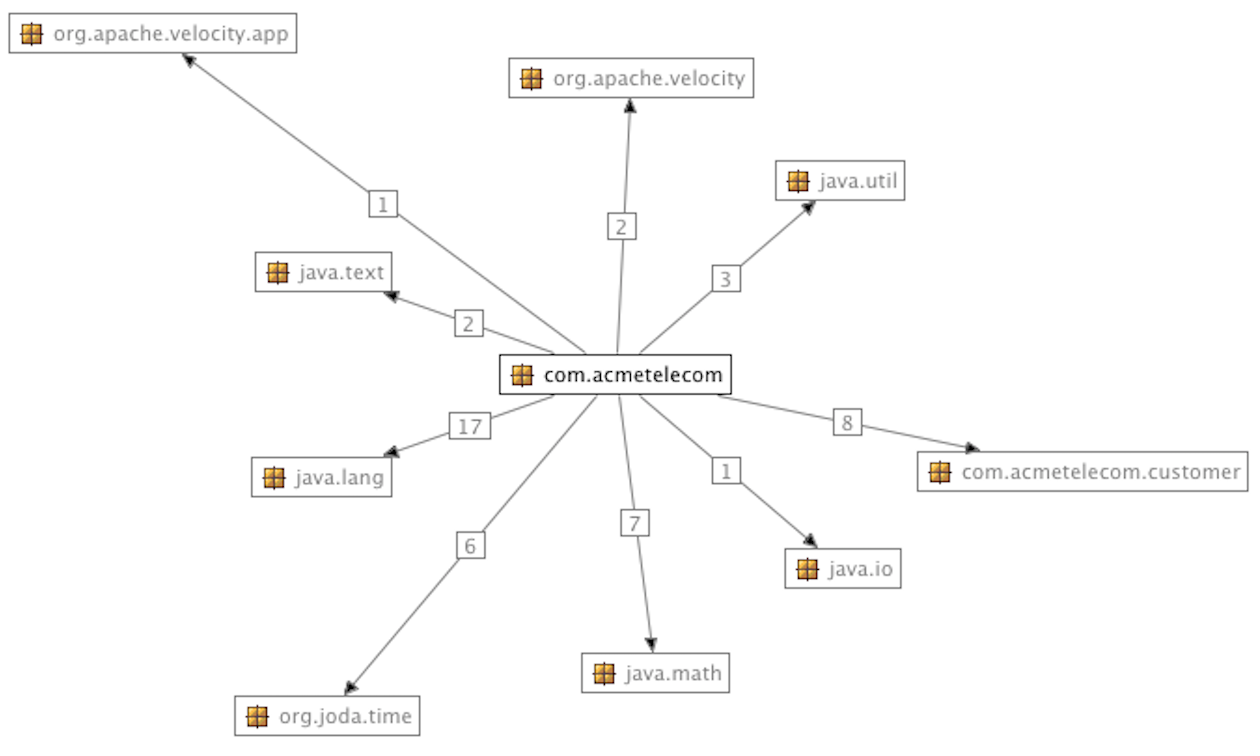
\includegraphics[scale=0.30]{overall_architecture.png}
\caption{Overall Architecture}
\end{figure}
Given this, we maintained BillingSystem as the root class of the system and delegated the above functionality to other classes whose
instances are injected into the BillingSystem instance.

Thus, the logging of events is represented through the CallLog interface. Currently, this is implemented using an Array.
The flexibility of the interface allows us to use another type of storage (Filesystem, database, cloud storage). 
We would like to point out that we have decided to use an iterator when reading through the logs. There is an increased 
performance when dealing with large amounts of data, because of the lazy loading of data.

Bill generation logic is encompassed in the BillingJob class. An important thing to note is how this class was written: its two methods, aggregateCalls
and createBill are the equivalent of the map and reduce functions respectively of a map reduce job. They can actually be reused to write a map-reduce
class, but they need to be wrapped by methods conforming to the Hadoop API. The reason behind this is to be able to handle large amounts of data
when scalability will be required.

The W3C standard in the HTML format is respected through the BillPrinter interface (allowing for other types of printing modes to be plugged in).
The current implementation, HTMLBillPrinter has been rewritten to make use of a templating library: Apache Velocity. The reason for this is to make
the representation more easily changeable and to minimize the code. Given the use of a template, we correctly split the design from the dynamic code generation
part in our application.

For the whole code, we followed the terms of the principle of purity, side-effects, I/O and testability although more as an inspiration since the
Java type system does not offer support for the above in the way other programming languages do (For ex: Haskell). Thus, we identified parts of the code which are
"pure" (ex. createBill) and made these methods stateless and dependent only on their parameters, since essentially they are just functions
that take an input and provide an output. This resulted in writing testes in a more modular fashion. 

\subsection{Removing the cyclic dependencies}
A cyclic dependency was by the inner class $LineItem$, which was placed inside the $BillingSystem.java$.
The $LineItem$ was used to store the customer's phone calls in a special data structure. In order to remove the cyclic dependency, we attached the
data contained by LineItem to the Call object.

In conclusion, the newly refactored code has no cyclic dependencies.

\section{Extra Work}
\subsection{Elastic Map Reduce}
\emph{Elastic MapReduce} or $EMR$ is an Amazon-based programming model used for processing very large data sets, 
having its behavior inspired from the functional programming functions $map$ and $reduce$. The overall process is well
documented in the computing literature.

We have provided an interface implementation for the ACME Telecom to use the power of $EMR$ when the system is needed to scale to 
accommodate more users. The main implementation is provided in the file $BillingMRJob.java$. Our implementation reads the list of calls and the 
customer information and starts a MapReduce job using Amazon $EMR$ in order to compute lightning-fast the costs for conversations used 
to generate the bills.

When the application will be required to scale and the number of customers for $AcmeTelecom$ will be very large, $EMR$ can be extremely 
helpful when computing the costs for conversations and generating the bills as fast as possible. The $EMR$ should be adequate for any 
scalability problems ACME Telecom might face in the future. Of course, out code is modular so \textit{AcmeTelecom} can choose any 
$EMR$ provider they like.

\begin{figure}[ht]
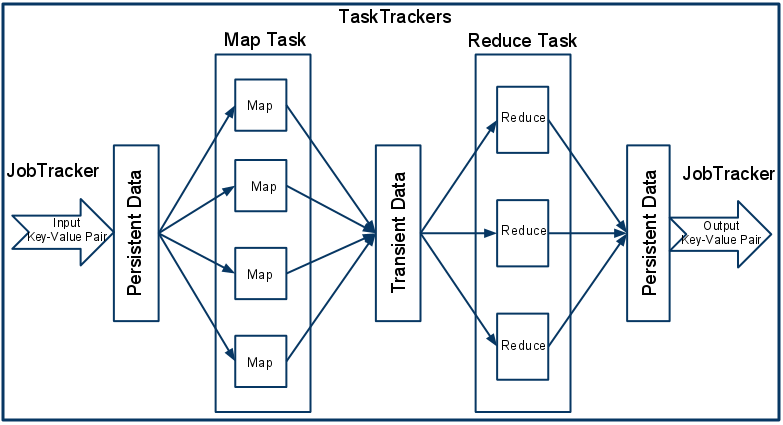
\includegraphics[scale=0.25]{hadoop.png}
\caption{Hadoop \cite{hadoop}}
\end{figure}

\subsection{Speed improvement}

In order to improve the run speed of our system, we have developed our algorithm to run in $\Theta$(n)
, where n is the length of the calls for each customer. We assert the fact that for each call,
the \textit{start} and \textit{end} times are chronologically ordered ( the \textit{end} call is \textbf{never}
before the \textit{start} call). Based on our assumption, we can then calculate in $\Theta$(1), for each call,
what is the total cost associated. 

\subsection{Source code validation}
Another important aspect of software engineering is source code validation. Besides the
aforementioned high level dependency analysis, we used tools like Lint4J
and CodePro AnalytiX to audit code, produce metrics (for ex: Afferent/Efferent Couplings), measure code quality, 
and find similar/dead code. The tools helped us streamline the codebase in preparation for deployment to a target environment.


\subsection{New Output Interface}
As discussed earlier, for 100\% legacy compatibility, we have decided to add new Classes extending the newly Output Interface. 
The first one we have added is the ConsolePrinter class that is used to print the BillingSystem output in a readable 
format used for debugging. This is what we have used to test our product, integrating the ConsolePrinter with the Tests we ran. 
Also, because our new system might be used part of a bigger architecture, we have decided to implement an API interface, 
used to export our system's data. We chose the REST JSON format as it is practical and is the most adopted format in the industry

\section{Testing}
Any new complex software has the potential to act in a different way than it was originally designed. As such, testing is \textit{essential} for any new piece of software 
so our approach was of a Test Driven Development (TDD) in order to make sure our system is developed as we intend it to work from the beginning. 

For this we came up with guides for implementation of the program logic and we made sure that the original design contract 
was implemented successfully when all the tests passed.            
Because of the number of tests, we decided to split tests into two packages: one for Unit Testing and one for Acceptance Testing.


\subsection{Unit Testing}

Unit tests can be found in the package com.acmetelecom.tests. Their primary purpose is to test components individually in isolation. 
Therefore, the Mockito\cite{mockito} framework has been used in order to help mock objects for the tests.

In order to asses our test coverage we have used the EMMA tool which produces a report describing classes, methods, blocks and lines tested. 
Since our initial code coverage was not good enough we use an automatic test generator for the rest of code: initialization of classes, methods calling with null arguments, etc. 
CodPro AnalytiX\cite{codePro}  is an automatic unit test generator tool that helped us make sure we have a very good test coverage and also spot any small issues with the code. 
For example, we identified and removed some unused references. Even though this might not seem very important for our application, it is a good practice because in a 
complex system it is important not to reference unused parts, since the system will carry information that is not needed and will increase its size in memory. This happens a lot with $DLLs$ in $C\#$. 

The output from a run using the EMMA tool can be seen below:

\begin{lstlisting}[language=bash]
java -cp emma.jar emmarun -jar softeng2.jar

[EMMA v2.0.5312 report, generated Tue Nov 19 19:57:47 GMT 2013]
-----------------------------------
OVERALL COVERAGE SUMMARY:

[class, %]   [method, %]    [block, %]   
100% (5/5)   79% (11/14)   89% (305/344) 

[line, %]    [name]
85% (67/79)  all classes
----------------------------------
\end{lstlisting}


\begin{figure}[!ht]
\centering
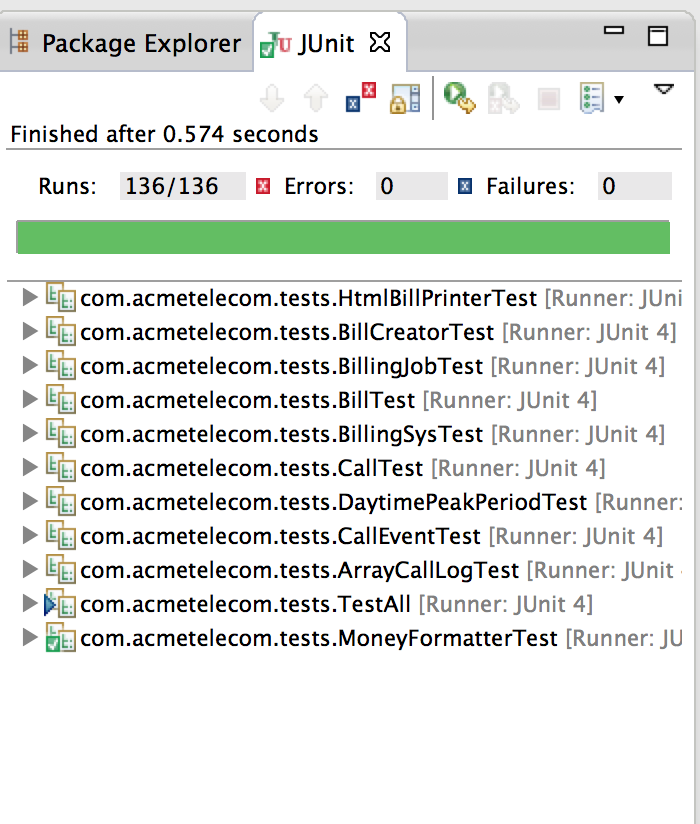
\includegraphics[scale=0.40]{cod_pro_analytix.png}
\caption{Unit Tests}
\end{figure}

\subsection{Acceptance Testing}
Acceptance testing is a test conducted to determine if the requirements of a specification or contract are met. 
It may involve chemical tests, physical tests, or performance tests.
In our case, the acceptance test is targetting the core class of this software which represents the system as whole, namely $BillingSystem$.
The actual test cases can be written by a non-programmer person because we make use of the Cucumber library, backed up by mockito.
Thus, one who would like to test our system would write scenarios in which they specify the call events followed by a description
of the textual html output expected from the bills.

\section{Software Engineering Practices}
During the implementation stage, good Software Development practices were maintained by the members of the group. 
We have extensively used some of the design patterns and development methodologies that we have learned during the implementation phase.

\subsection{Project Management}
Managing the project was a crucial aspect throughout the entire period. The group had regular Scrum meetings in order to discuss the 
progress of the project, where the team-members were brainstorming sessions, draw sketches of different scenarios, looked at
what could actually be done with the existing source code and what improvements will be necessary. All decisions were taken
within the majority of the group members.

\subsection{Design Patterns Used}
During the code refactoring stage, we have made extensive use of design patterns.
\begin{itemize}
\item{{\bf Iterator pattern} provides a way to access the elements of an aggregate object sequentially. We have used this pattern ($BillCreator.java$).}
\item{{\bf Prototype pattern}  create new objects objects create using a prototype. The $HTMLBillTemplate.vm$ is a template used to create $HTMLBillPrinter.java$}
\item{{\bf Strategy pattern} defines a family of algorithms, encapsulate each one, and make them interchangeable. The classes $ConsolePrinter.java$ and $HTMLBillPrinter$ exemplify this pattern in our code.}
\end{itemize}


\subsection{Agile Development}
The group has decided to use an \emph{iterative approach} in order to add value to our project from the beginning. 
Refactoring allowed us to change the internal structure of our code without interfering with its external behaviour. While trying to reduce complexity, refactoring continuously improved the design of the source code, reducing the complexity of our task.
Communication was also a vital factor when working for this project. The strong relationship among the developers made the task both 
easier and enjoyable.

\section{Conclusion}
In conclusion, we present a solution that makes use of the appropriate software engineering practices, in order to 
make sure that the whole system behaves correctly.
The main logic of our solution is encapsulated in the $BillingJob.java$ and it works for pricing phone calls longer than $24$ hours. 
The code was properly refactored in order to make it easy to understand its functionality and it was tested properly.
An automated testing tool ($AnalitiX$ $CodePro$) was used to generate the unit tests.
The resulting coverage for the classes was $100\%$ and $79\%$ for methods.
In extension to the traditional tasks, the team has agreed to implement an extension for the $AWS$ $Elastic$ $Map$ $Reduce$ that is runnable on $Hadoop$.

\begin{thebibliography}{9}
\bibitem{mockito}
  \emph{Mockito}.
  http://docs.mockito.google\\code.com/hg/org/mockito/Mockito.html  

\bibitem{JUnit}
  \emph{JUnit}.
  https://github.com/junit-team/junit/wiki

\bibitem{UncleBob}
  \emph{Design Principles and Design Patterns}.
  Robert C. Martin,
  2000

\bibitem{hadoop}
  \emph{Hadoop}.
  http://thetechmusings.files.wordpress.com/2011/\\02/hadoop-mapreduce-execution-framework.png
  
\bibitem{codePro}
  \emph{CodePro AnalitiX}.
  https://developers.google.com/java-dev-tools/codepro/doc/ 
  
\end{thebibliography}




\end{document}          
